\documentclass[12pt]{article}
\usepackage{fancyhdr}
\usepackage{amsmath,amsfonts,enumerate}
\usepackage{color,graphicx}
\usepackage{tikz}
\usepackage{pgfplots}
\usepackage{listings}
\usepackage{algorithm}
\usepackage{algorithmic}
\usetikzlibrary{arrows,positioning,shapes,calc,matrix}
\pagestyle{fancy}
%%%%%%%%%%%%%%%%%%%%%%%%%%%%%%%%%%%%%%%%%%%%%%%%%
% Course customization based on university sources
%%%%%%%%%%%%%%%%%%%%%%%%%%%%%%%%%%%%%%%%%%%%%%%%%
\newcommand{\masunitnumber}{CENG 403}
\newcommand{\examdate}{January 2025}
\newcommand{\academicyear}{2024-2025}
\newcommand{\semester}{I}
\newcommand{\coursename}{Deep Learning - RNNs, LSTM \& Language Models (University Sources)}
\newcommand{\numberofhours}{3}
%%%%%%%%%%%%%%%%%%%%%%%%%%%%%%%%%%%%%%%%%%%%%%%%%
% CUSTOM SPACING COMMANDS FOR ANSWER SPACES
%%%%%%%%%%%%%%%%%%%%%%%%%%%%%%%%%%%%%%%%%%%%%%%%%
\newcommand{\answerspace}[1]{\vspace{#1}}
\newcommand{\questionspace}{\vspace{3cm}}        
\newcommand{\subquestionspace}{\vspace{2.5cm}}   
\newcommand{\shortanswer}{\vspace{2cm}}          
\newcommand{\mediumanswer}{\vspace{3cm}}         
\newcommand{\longanswer}{\vspace{4cm}}           
\newcommand{\journalspace}{\vspace{4.5cm}}       
\newcommand{\codespace}{\vspace{5cm}}            
%%%%%%%%%%%%%%%%%%%%%%%%%%%%%%%%%%%%%%%%%%%%%%%%%
% Header setup
%%%%%%%%%%%%%%%%%%%%%%%%%%%%%%%%%%%%%%%%%%%%%%%%%
\lhead{}
\rhead{}
\chead{{\bf MIDDLE EAST TECHNICAL UNIVERSITY}}
\lfoot{}
\rfoot{}
\cfoot{}
\begin{document}
\setlength{\headsep}{5truemm}
\setlength{\headheight}{14.5truemm}
\setlength{\voffset}{-0.45truein}
\renewcommand{\headrulewidth}{0.0pt}
\begin{center}
SEMESTER \semester\ EXAMINATION \academicyear
\end{center}
\begin{center}
{\bf \masunitnumber\ -- \coursename}
\end{center}
\vspace{20truemm}
\noindent \examdate\hspace{45truemm} TIME ALLOWED: \numberofhours\ HOURS
\vspace{19truemm}
\hrule
\vspace{19truemm}
\noindent\underline{INSTRUCTIONS TO CANDIDATES}
\vspace{8truemm}
%%%%%%%%%%%%%%%%%%%%%%%%%%%%%%%%%%%%%%%%%%%%%%%%%%%%%%
% Instructions based on university standards
%%%%%%%%%%%%%%%%%%%%%%%%%%%%%%%%%%%%%%%%%%%%%%%%%%%%%%
\begin{enumerate}
\item This examination paper contains {\bf SEVEN (7)} questions and comprises 
{\bf TEN (10)} printed pages.
\item Answer all questions. 
The marks for each question are indicated at the beginning of each question.
\item Answer each question beginning on a {\bf FRESH} page of the answer book.
\item This {\bf IS NOT an OPEN BOOK} exam.
\item Show all mathematical derivations clearly with proper notation.
\item For implementation questions, provide clear pseudocode or algorithms.
\item Explain computational complexity where requested.
\item Draw clear architectural diagrams with proper labels.
\end{enumerate}
%%%%%%%%%%%%%%%%%%%%%%%%%%%%%%%%%%%%%%%%%%%%%%%%%
% New page for questions
%%%%%%%%%%%%%%%%%%%%%%%%%%%%%%%%%%%%%%%%%%%%%%%%%
\newpage
\lhead{}
\rhead{\masunitnumber}
\chead{}
\lfoot{}
\cfoot{\thepage}
\rfoot{}
\setlength{\footskip}{45pt}
%%%%%%%%%%%%%%%%%%%%%%%%%%%%%%%%%%%%%%%%%%%%%%%%%%
% EXAM QUESTIONS BASED ON UNIVERSITY SOURCES
%%%%%%%%%%%%%%%%%%%%%%%%%%%%%%%%%%%%%%%%%%%%%%%%%%

\paragraph{Question 1. Backpropagation Through Time (BPTT)}\hfill (25 marks)\\
Based on Stanford/MIT/University of Toronto deep learning courses.

\begin{enumerate}[(a)]
    \item Define Backpropagation Through Time (BPTT) and explain how it extends traditional backpropagation to sequential data. Include the mathematical formulation for unfolding an RNN across time steps. \hfill (8 marks)
    
    \mediumanswer
    
    \item Consider an RNN with hidden state update equation: \hfill (12 marks)
    $$h_t = \tanh(W_{hx} x_t + W_{hh} h_{t-1} + b_h)$$
    $$y_t = W_{hy} h_t + b_y$$
    
    For a sequence of length T=3, derive the gradient $\frac{\partial L}{\partial W_{hh}}$ where $L = \sum_{t=1}^3 L_t$ is the total loss. Show the complete gradient computation including the chain rule applications.
    
    \journalspace
    
    \item Explain truncated BPTT and why it's necessary for long sequences. Compare regular truncation vs. randomized truncation approaches, discussing computational complexity and numerical stability. \hfill (5 marks)
    
    \mediumanswer
\end{enumerate}

\newpage
\paragraph{Question 2. LSTM Architecture and Gating Mechanisms}\hfill (30 marks)\\
Based on university deep learning course materials and D2L.ai educational content.

\begin{enumerate}[(a)]
    \item Draw the complete LSTM cell architecture showing all gates (input, forget, output) and state components (cell state, hidden state). Label all weight matrices and explain information flow. \hfill (10 marks)
    
    \begin{center}
    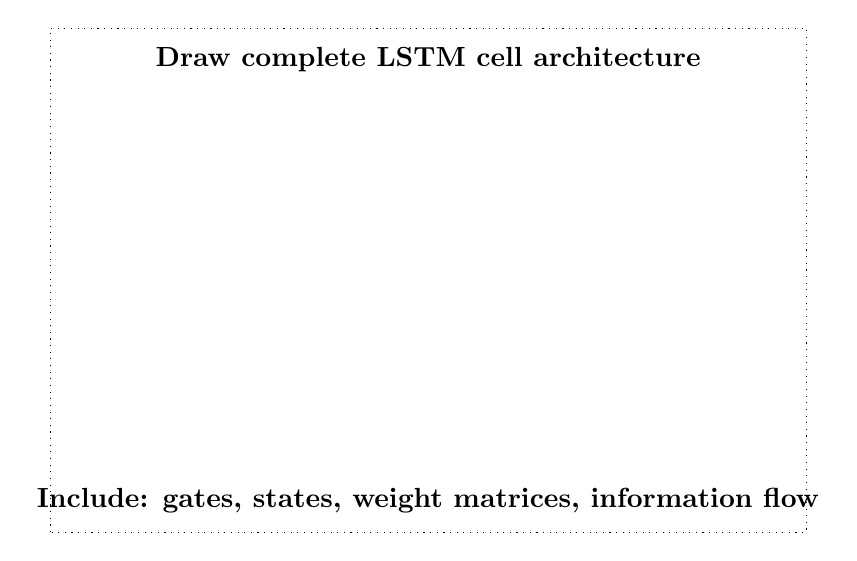
\begin{tikzpicture}[scale=0.8]
        % Space for LSTM architecture drawing
        \draw[dotted] (0,0) rectangle (12,8);
        \node at (6,7.5) {\textbf{Draw complete LSTM cell architecture}};
        \node at (6,0.5) {\textbf{Include: gates, states, weight matrices, information flow}};
    \end{tikzpicture}
    \end{center}
    
    \shortanswer
    
    \item Write the mathematical equations for all LSTM gates and state updates. Given input $x_t$, previous hidden state $h_{t-1}$, and previous cell state $C_{t-1}$, derive: \hfill (15 marks)
    \begin{itemize}
        \item Forget gate: $f_t = ?$
        \item Input gate: $i_t = ?$
        \item Candidate values: $\tilde{C}_t = ?$
        \item Cell state update: $C_t = ?$
        \item Output gate: $o_t = ?$
        \item Hidden state: $h_t = ?$
    \end{itemize}
    
    \journalspace
    
    \item Compare LSTM vs. vanilla RNN in terms of gradient flow. Explain how the cell state pathway in LSTM addresses the vanishing gradient problem through mathematical analysis of gradient propagation. \hfill (5 marks)
    
    \mediumanswer
\end{enumerate}

\newpage
\paragraph{Question 3. Word Embeddings and Distributional Semantics}\hfill (22 marks)\\
Based on NLP course materials from Stanford CS224n and similar university programs.

\begin{enumerate}[(a)]
    \item Explain the distributional hypothesis that underlies word embeddings. How does the CBOW (Continuous Bag of Words) model implement this principle? \hfill (6 marks)
    
    \mediumanswer
    
    \item Design the Skip-gram model architecture for learning word embeddings. Given vocabulary size V=10,000 and embedding dimension d=300: \hfill (10 marks)
    \begin{itemize}
        \item Draw the network architecture
        \item Calculate the number of parameters
        \item Explain the softmax bottleneck and hierarchical softmax solution
        \item Derive the loss function using negative sampling
    \end{itemize}
    
    \journalspace
    
    \item Analyze word embedding arithmetic: "king - man + woman ≈ queen". Explain: \hfill (6 marks)
    \begin{itemize}
        \item Why this works mathematically in embedding space
        \item What linguistic relationships are captured
        \item Limitations of linear analogies in embeddings
    \end{itemize}
    
    \mediumanswer
\end{enumerate}

\newpage
\paragraph{Question 4. Sequence-to-Sequence Models and Attention}\hfill (28 marks)\\
Based on modern NLP course materials covering encoder-decoder architectures.

\begin{enumerate}[(a)]
    \item Design an encoder-decoder RNN architecture for machine translation from English to French. Show the complete architecture including: \hfill (12 marks)
    \begin{itemize}
        \item Encoder RNN processing input sequence
        \item Context vector computation
        \item Decoder RNN generating output sequence
        \item How teacher forcing works during training
        \item Inference procedure using greedy/beam search
    \end{itemize}
    
    \journalspace
    
    \item Implement beam search decoding with beam size k=3. Given the following probability distributions over vocabulary {A, B, C, \textless EOS\textgreater} for 2 time steps: \hfill (10 marks)
    
    \begin{center}
    \begin{tabular}{|c|c|c|c|c|}
    \hline
    Context & P(A) & P(B) & P(C) & P(\textless EOS\textgreater) \\
    \hline
    Initial & 0.5 & 0.3 & 0.15 & 0.05 \\
    After A & 0.2 & 0.1 & 0.6 & 0.1 \\
    After B & 0.4 & 0.2 & 0.3 & 0.1 \\
    After C & 0.1 & 0.7 & 0.1 & 0.1 \\
    \hline
    \end{tabular}
    \end{center}
    
    Show the complete beam search tree and final ranked sequences.
    
    \codespace
    
    \item Explain the attention mechanism as a solution to the bottleneck problem in sequence-to-sequence models. Derive the mathematical formulation for Bahdanau attention. \hfill (6 marks)
    
    \mediumanswer
\end{enumerate}

\newpage
\paragraph{Question 5. Gradient Problems and Solutions}\hfill (20 marks)\\
Based on theoretical analysis from university deep learning courses.

\begin{enumerate}[(a)]
    \item Analyze the vanishing gradient problem in RNNs. For an RNN with hidden state transition $h_t = \tanh(W h_{t-1} + U x_t)$, show mathematically why gradients vanish for long sequences. \hfill (8 marks)
    
    Include analysis of:
    \begin{itemize}
        \item Gradient computation through multiple time steps
        \item Effect of tanh derivative bounds
        \item Impact of weight matrix eigenvalues
    \end{itemize}
    
    \mediumanswer
    
    \item Compare three solutions to gradient problems in RNNs: \hfill (12 marks)
    \begin{itemize}
        \item Gradient clipping (explain algorithm and threshold selection)
        \item LSTM gating mechanisms (focus on gradient flow)
        \item Skip connections in deep RNNs
    \end{itemize}
    
    Provide mathematical justification for each approach.
    
    \longanswer
\end{enumerate}

\newpage
\paragraph{Question 6. Language Modeling Evaluation and Perplexity}\hfill (18 marks)\\
Based on NLP evaluation metrics taught in university courses.

\begin{enumerate}[(a)]
    \item Define perplexity as a measure of language model quality. Given a test sequence $w_1, w_2, \ldots, w_N$, derive the relationship between perplexity and cross-entropy loss. \hfill (8 marks)
    
    \mediumanswer
    
    \item A character-level RNN language model with vocabulary size 50 achieves the following results: \hfill (10 marks)
    \begin{itemize}
        \item Training perplexity: 1.8
        \item Validation perplexity: 2.3
        \item Test perplexity: 2.5
    \end{itemize}
    
    \begin{itemize}
        \item Calculate the average bits per character for each dataset
        \item Analyze what these results indicate about model performance
        \item Compare with a baseline uniform model (calculate its perplexity)
        \item Suggest improvements to reduce the validation-test gap
    \end{itemize}
    
    \mediumanswer
\end{enumerate}

\newpage
\paragraph{Question 7. Modern RNN Variants and Applications}\hfill (27 marks)\\
Based on advanced topics from recent university deep learning curricula.

\begin{enumerate}[(a)]
    \item Compare GRU (Gated Recurrent Unit) with LSTM architecture. Draw both architectures and explain: \hfill (12 marks)
    \begin{itemize}
        \item Key architectural differences
        \item Parameter count comparison
        \item Computational efficiency analysis
        \item When to choose GRU vs LSTM
    \end{itemize}
    
    \journalspace
    
    \item Design a bidirectional RNN for named entity recognition. Explain: \hfill (8 marks)
    \begin{itemize}
        \item Forward and backward pass computations
        \item How to combine directional information
        \item Advantages for sequence labeling tasks
        \item Training considerations
    \end{itemize}
    
    \mediumanswer
    
    \item Analyze the computational complexity of different RNN variants: \hfill (7 marks)
    
    \begin{center}
    \begin{tabular}{|l|c|c|c|}
    \hline
    Model & Time Complexity & Space Complexity & Parameters \\
    \hline
    Vanilla RNN & ? & ? & ? \\
    LSTM & ? & ? & ? \\
    GRU & ? & ? & ? \\
    Bidirectional LSTM & ? & ? & ? \\
    \hline
    \end{tabular}
    \end{center}
    
    For sequence length T, hidden size H, and input size D.
    
    \shortanswer
\end{enumerate}

\vfill
\begin{center}{\bf END OF PAPER}\end{center>
\end{document}